\usepackage{pgf}
\usepackage{tikz}
\usetikzlibrary{arrows,automata,fit, shapes, calc}

\tikzstyle{inputNode}=[draw=white,circle,minimum size=10pt,inner sep=0pt]
\tikzstyle{stateTransition}=[->, thick]
\def\layersep{2.5cm}

\tikzset{
	every node/.style={
		font=\scriptsize
	},
	dinero/.style={
		shape=rectangle,
		minimum height=1cm,
		text width=2cm,
		text centered,
		rounded corners=1ex,
		draw,
		label={[yshift=-0.7cm]left:poco},
		label={[yshift=-0.7cm]right:mucho},
	},
	tiempo/.style={
		shape=rectangle,
		minimum height=1cm,
		text width=2cm,
		text centered,
		rounded corners=1ex,
		draw,
		label={[yshift=-0.7cm]left:soleado},
		label={[yshift=-0.7cm]right:lluvioso},
	},
	outcome/.style={
		shape=ellipse,
		fill=gray!15,
		draw,
		text width=1.5cm,
		text centered
	},
	decision tree/.style={
		edge from parent path={[-latex] (\tikzparentnode) -| (\tikzchildnode)},
		sibling distance=3cm,
		level distance=1.125cm
	}
}

\tikzset{
	every node/.style={
		font=\scriptsize
	},
	moroso/.style={
		shape=rectangle,
		minimum height=1cm,
		text width=2cm,
		text centered,
		rounded corners=1ex,
		draw,
		label={[yshift=-0.7cm]left:sí},
		label={[yshift=-0.7cm]right:no},
	},
	ingresos/.style={
		shape=rectangle,
		minimum height=1cm,
		text width=2cm,
		text centered,
		rounded corners=1ex,
		draw,
		label={[yshift=-0.25cm]left:$<600$},
		label={[yshift=-0.25cm]right:$600-1200$},
		label={[yshift=-0.1cm, xshift=0.5cm]below:$>1200$},
	},
	outcome/.style={
		shape=ellipse,
		fill=gray!15,
		draw,
		text width=1.5cm,
		text centered
	},
	decision tree/.style={
		edge from parent path={[-latex] (\tikzparentnode) -- (\tikzchildnode)},
		sibling distance=3cm,
		level distance=1.125cm
	}
}

\tikzset{
	every node/.style={
		font=\scriptsize
	},
	node/.style={
		shape=rectangle,
		minimum height=1cm,
		text width=2cm,
		text centered,
		rounded corners=1ex,
		draw,
	},
	myarrow/.style={->},
	myarrow2/.style={<-},        
}

\newcommand{\arboldedecision}{
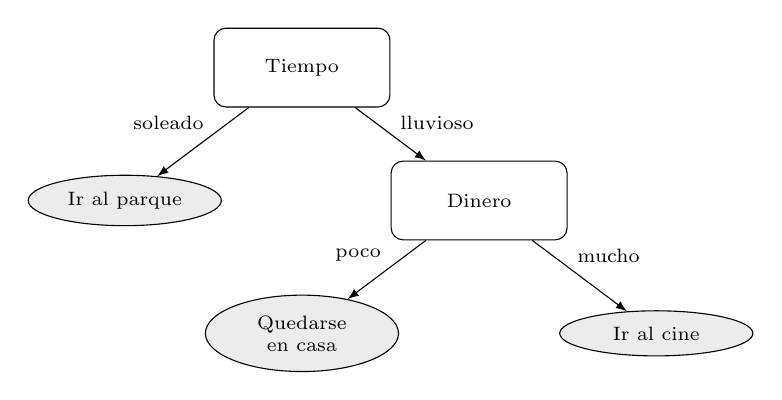
\begin{tikzpicture}[scale = 1.5]
\node [tiempo] {Tiempo }
[decision tree]
child { node [outcome] {Ir al parque} }
child { node [dinero] { Dinero } 
	child { node [outcome] { Quedarse en casa } }
	child { node [outcome] { Ir al cine } }
};
\end{tikzpicture}	
}

\newcommand{\ejemploarboldecision}{
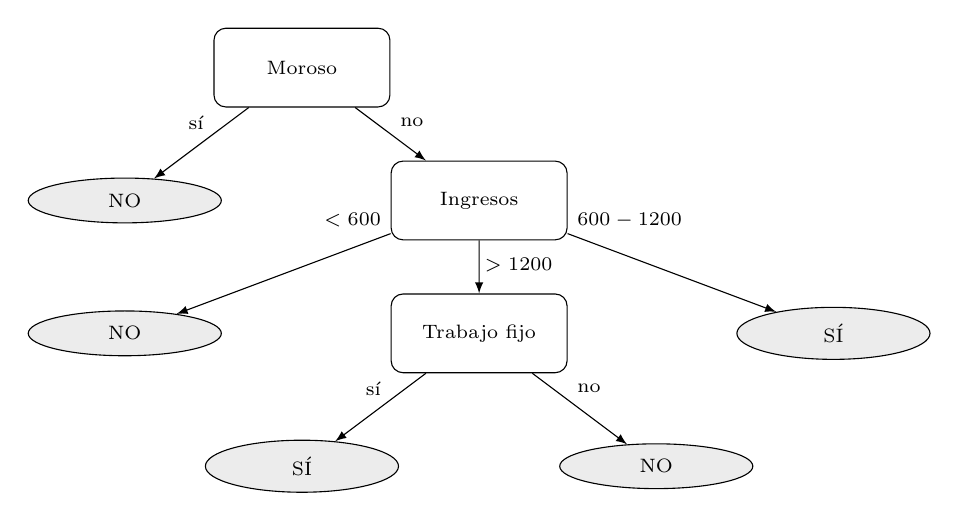
\begin{tikzpicture}[scale = 1.5]

\node [moroso] {Moroso}[decision tree]
child { node [outcome] {NO} }
child { node [ingresos] { Ingresos } 
	child { node [outcome] { NO } }
	child { node [moroso] {Trabajo fijo}
		child { node [outcome] { SÍ } }
		child { node [outcome] { NO } }
	}
	child { node [outcome] { SÍ } }
};

\end{tikzpicture}	
}

\newcommand{\ejemplografo}{
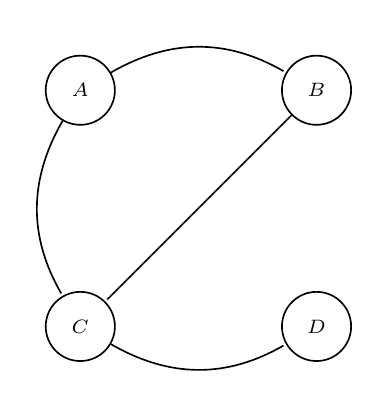
\begin{tikzpicture}[>=stealth',shorten >=1pt,auto,node distance=3cm,semithick]
  \tikzstyle{every state}=[draw=black,text=black]

  \node[state]         (A)                    {$A$};
  \node[state]         (B) [right of=A]       {$B$};
  \node[state]         (C) [below of=A]       {$C$};
  \node[state]         (D) [right of=C]       {$D$};
  
  \path (A) edge  [bend left]   node {}  (B)
            edge  [bend right]  node {}  (C)
        (B) edge                node {}  (C)
        (C) edge  [bend right]  node {}  (D);
\end{tikzpicture}}

\newcommand{\neuronaMcCullochPitts}{
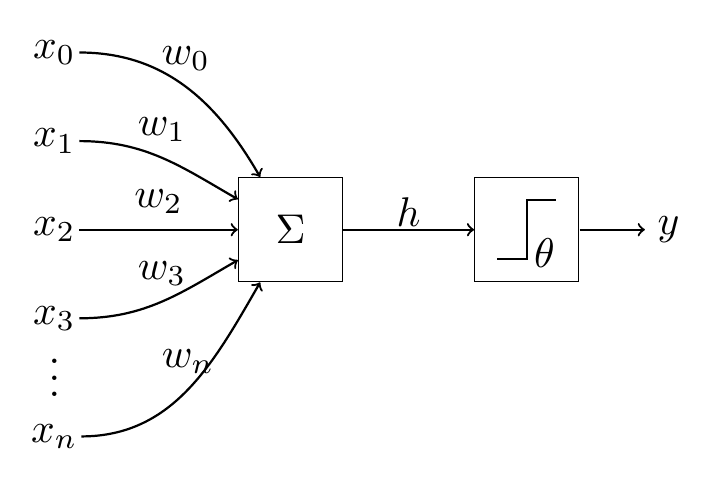
\begin{tikzpicture}[scale=1.5, every node/.style={scale=1.5}]
\node[draw,minimum size=25pt,inner sep=0pt] (x) at (0,0) {$\Sigma$};
\node[draw,minimum size=25pt,inner sep=0pt] (s) at (2,0) {};

\node[inputNode] (x0) at (-2, 1.5) {$x_0$};
\node[inputNode] (x1) at (-2, 0.75) {$x_1$};
\node[inputNode] (x2) at (-2, 0) {$x_2$};
\node[inputNode] (x3) at (-2, -0.75) {$x_3$};
\node[inputNode] (xn) at (-2, -1.75) {$x_n$};

\draw[stateTransition] (x0) to[out=0,in=120] node [above=0.1]  {$w_0$} (x);
\draw[stateTransition] (x1) to[out=0,in=150] node [above=0.1] {$w_1$} (x);
\draw[stateTransition] (x2) to[out=0,in=180] node [above=0.1] {$w_2$} (x);
\draw[stateTransition] (x3) to[out=0,in=210] node [above=0.1] {$w_3$} (x);
\draw[stateTransition] (xn) to[out=0,in=240] node [above=0.1] {$w_n$} (x);

\draw[stateTransition] (x) -- (s) node [midway,above=-0.1cm] {$h$};
\draw[stateTransition] (s) -- (3,0) node [midway,above=-0.1cm] {};
\node[draw=none] at (3.2,0) {$y$};

\node (dots) at (-2, -1.15) {$\vdots$};

\draw[thick] (1.75,-0.25) -- (2,-0.25) -- (2, 0.25) -- (2.25,0.25);
\node[draw=none] at (2.15,-0.2) {$\theta$};
\end{tikzpicture}
}

\newcommand{\perceptron}{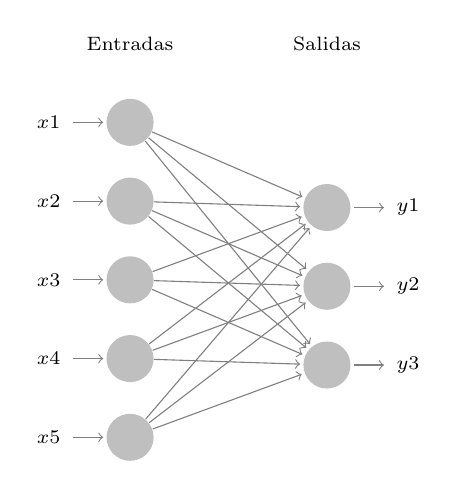
\begin{tikzpicture}
	[shorten >=1pt,->,draw=black!50, node distance=\layersep]
	\tikzstyle{every pin edge}=[<-,shorten <=1pt]
	\tikzstyle{neuron}=[circle,fill=gray!25,minimum size=17pt,inner sep=0pt]
	\tikzstyle{input neuron}=[neuron, fill=gray!50];
	\tikzstyle{output neuron}=[neuron, fill=gray!50];
	\tikzstyle{hidden neuron}=[neuron, fill=gray!50];
	\tikzstyle{annot} = [text width=4em, text centered]
	
	\foreach \name / \y in {1,...,5}
	\node[input neuron, pin=left: $x$\y] (I-\name) at (0,-\y) {};
	
	\foreach \name / \y in {1,...,3}
	\path[yshift=0.5cm]
	node[hidden neuron,pin={[pin edge={->}]right:$y$\y}] (O-\name) at (\layersep,-45-\y cm) {};
	
	\foreach \source in {1,...,5}
	\foreach \dest in {1,...,3}
	\path (I-\source) edge (O-\dest);
	
	\node[annot,above of=I-1, node distance=1cm] (hl) {Entradas};
	\node[annot,right of=hl] {Salidas};
\end{tikzpicture}}

\newcommand{\linealmenteseparable}{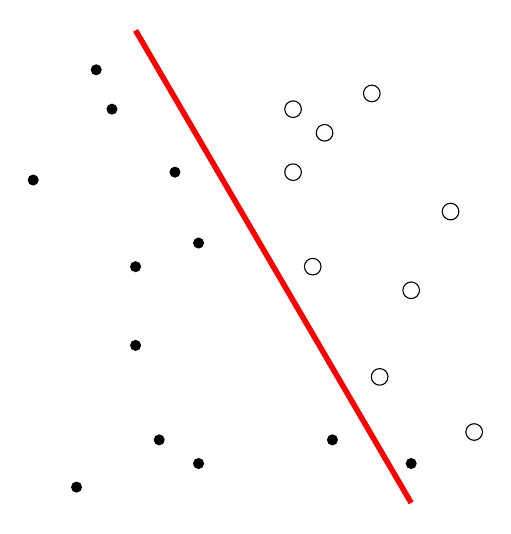
\begin{tikzpicture}
	
	\draw[color=red,line width=2pt] (8.5,6) -- (12,0);
	
	\def\positive{{%
			{9.3,3.3},
			{11,.8},
			{8.5,2},
			{7.2,4.1},
			{8.8,.8},
			{8,5.5},
			{8.2,5},
			{7.75,.2},
			{9,4.2},
			{12, 0.5},
			{8.5,3},
			{9.3,.5},
		}}
		
		\foreach \i in {0,...,11} {
			\pgfmathparse{\positive[\i][0]}\let \x \pgfmathresult;
			\pgfmathparse{\positive[\i][1]}\let \y \pgfmathresult;
			\fill[black] (\x,\y) circle (2pt);
		}
		
		\def\negative{{%
				{10.75,3},
				{10.5,5},
				{11.6,1.6},
				{11.5,5.2},
				{12.5,3.7},
				{10.9,4.7},
				{12,2.7},
				{10.5,4.2},
				{12.8,.9},
			}}
			
			\foreach \i in {0,...,8} {
				\pgfmathparse{\negative[\i][0]}\let \x \pgfmathresult;
				\pgfmathparse{\negative[\i][1]}\let \y \pgfmathresult;
				\draw[black] (\x,\y) circle (3pt);
			}
			
			\end{tikzpicture}}
		
\newcommand{\nolinealmenteseparable}{	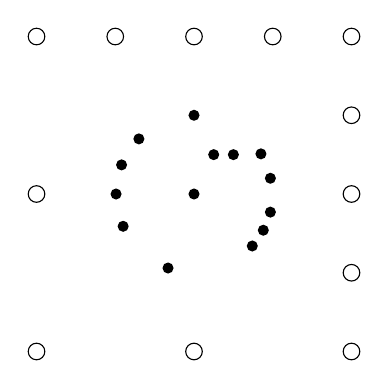
\begin{tikzpicture}
	
	\def\positive{{%
			{0.97,-0.23},
			{-0.33,-0.94},
			{-0.9,-0.41},
			{0.74,-0.66},
			{0.97,0.20},
			{0.88,-0.46},
			{-0.70,0.70},
			{-0.92,0.37},
			{0.85,0.51},
			{-0.99, 0},
			{0,0},
			{0.5,0.5},
			{0,1},
			{0.25, 0.5}
		}}
		
		\foreach \i in {0,...,13} {
			\pgfmathparse{\positive[\i][0]}\let \x \pgfmathresult;
			\pgfmathparse{\positive[\i][1]}\let \y \pgfmathresult;
			\fill[black] (\x,\y) circle (2pt);
		}
		
		\def\negative{{%
				{2,1},
				{1,2},
				{0,2},
				{-1,2},
				{2,-1},
				{2,0},
				{-2,0},
				{-2,-2},
				{0,-2},
				{-2,2},
				{2,2},
				{2,-2}
			}}
			
			\foreach \i in {0,...,11} {
				\pgfmathparse{\negative[\i][0]}\let \x \pgfmathresult;
				\pgfmathparse{\negative[\i][1]}\let \y \pgfmathresult;
				\draw[black] (\x,\y) circle (3pt);
			}
			
			\end{tikzpicture}}

\newcommand{\xor}{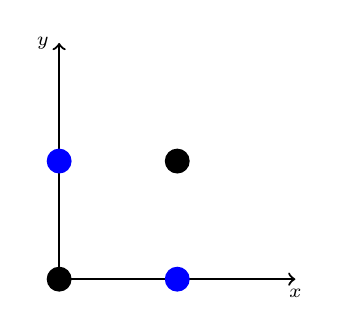
\begin{tikzpicture}[scale=1.5]
	
	\draw [<->,thick] (0,2) node (yaxis) [left] {$y$}
	|- (2,0) node (xaxis) [below] {$x$};
	
	\fill[black] (0,0) circle (3pt);
	\fill[blue] (1,0) circle (3pt);
	\fill[blue] (0,1) circle (3pt);
	\fill[black] (1,1) circle (3pt);
	\end{tikzpicture}}

\newcommand{\perceptronmulticapa}{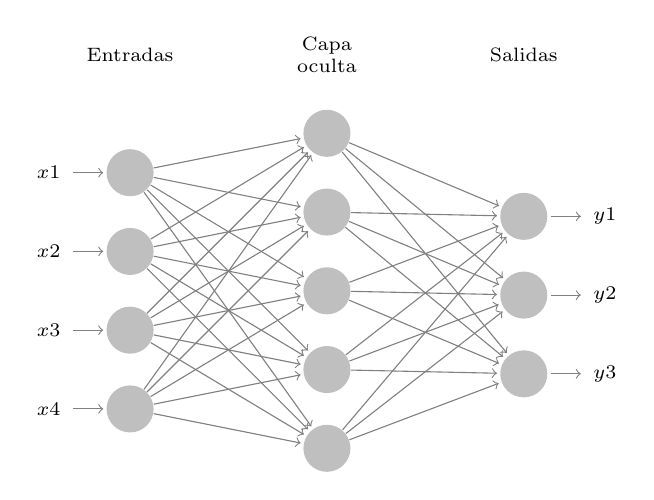
\begin{tikzpicture}
	[shorten >=1pt,->,draw=black!50, node distance=\layersep]
	\tikzstyle{every pin edge}=[<-,shorten <=1pt]
	\tikzstyle{neuron}=[circle,fill=gray!25,minimum size=17pt,inner sep=0pt]
	\tikzstyle{input neuron}=[neuron, fill=gray!50];
	\tikzstyle{output neuron}=[neuron, fill=gray!50];
	\tikzstyle{hidden neuron}=[neuron, fill=gray!50];
	\tikzstyle{annot} = [text width=4em, text centered]
	
	\foreach \name / \y in {1,...,4}
	\node[input neuron, pin=left: $x$\y] (I-\name) at (0,-\y) {};
	
	\foreach \name / \y in {1,...,5}
	\path[yshift=0.5cm]
	node[hidden neuron] (H-\name) at (\layersep,-\y cm) {};
	
	\foreach \name / \y in {1,...,3}
	\path[yshift=0.5cm]
	node[hidden neuron,pin={[pin edge={->}]right:$y$\y}] (O-\name) at (2*\layersep,-30-\y cm) {};
	
	\foreach \source in {1,...,4}
	\foreach \dest in {1,...,5}
	\path (I-\source) edge (H-\dest);
	
	\foreach \source in {1,...,5}
	\foreach \dest in {1,...,3}
	\path (H-\source) edge (O-\dest);
	
	\node[annot,above of=H-1, node distance=1cm] (hl) {Capa oculta};
	\node[annot,left of=hl] {Entradas};
	\node[annot,right of=hl] {Salidas};
\end{tikzpicture}}

\newcommand{\aprendizajerefuerzo}{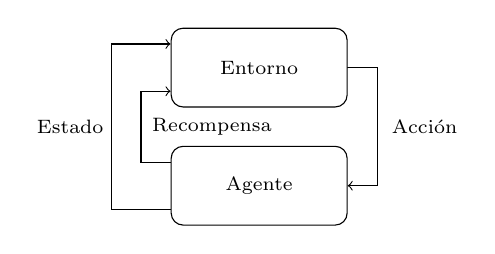
\begin{tikzpicture}[scale = 1.5]
	\node [node] (agt) at (0,1) {Entorno};
	\node [node] (ent) at (0,0) {Agente};
	\draw [myarrow2] (ent.east) -- ++(.25,0) -- ++(0,1) -|  (agt.east);		
	\draw [myarrow] (-0.75, 0.2) -- (-1,0.2) -- (-1,0.8) -- (-0.75,0.8);
	\draw [myarrow] (-0.75,-0.2) -- (-1.25,-0.2) -- (-1.25,1.2) -- (-0.75,1.2);
	
	\node[draw=none] at (1.4,0.5) {Acción};
	\node[draw=none] at (-0.4,0.5) {Recompensa};
	\node[draw=none] at (-1.6,0.5) {Estado};
	
	
	\end{tikzpicture}}